% 2011 年山东卷文科第 19 题：四棱台 ABCD-A1B1C1D1。
% 来源 PDF：普通高考/2011/2011山东文.pdf，SHA-256 bf61cf7bb39a3ccfc57735cd2a7ab34387cbfa6bc86a5e7f8246e13292b0e023。
% 原页：第 2 页（A3 三栏）第 1 栏下部，书页码 692。
% 重绘依据：按原页矢量层逐棱实测复刻。坐标取原页 pt：X = x_页 − 254.98，Y = 588.50 − y_页。
%   底面 ABCD（下底）：A(0,0)、B(102.01,0)、C(134.66,26.52)、D(32.64,26.52)；
%   上底 A1B1C1D1：A1(13.52,49.98)、B1(71.41,49.98)、C1(90.54,64.78)、D1(32.64,64.78)。
%   实线：AB、BC、CC1、C1D1、D1A1、A1A、A1B1、B1C1、B1B、A1B；
%   虚线：DA、DC、DB、DA1、DD1（D 与三条被遮挡的棱，原页不画顶点圆点、不标直角）。
%   原页 D 处的虚线交点处有一小叉，属虚线交叉，不另画。
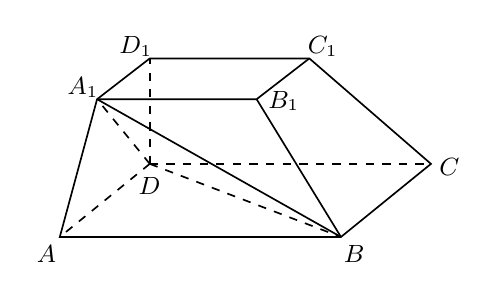
\begin{tikzpicture}[x=0.035cm, y=0.035cm, >=stealth, semithick, font=\small]
  % ===== 顶点 =====
  \coordinate (A)  at (0,0);
  \coordinate (B)  at (102.01,0);
  \coordinate (C)  at (134.66,26.52);
  \coordinate (D)  at (32.64,26.52);
  \coordinate (A1) at (13.52,49.98);
  \coordinate (B1) at (71.41,49.98);
  \coordinate (C1) at (90.54,64.78);
  \coordinate (D1) at (32.64,64.78);

  % ===== 可见的棱（实线） =====
  \draw (A) -- (B) -- (C) -- (C1) -- (D1) -- (A1) -- cycle;
  \draw (A1) -- (B1) -- (C1);
  \draw (B1) -- (B);
  \draw (A1) -- (B);

  % ===== 被遮挡的棱（虚线） =====
  \draw[dashed] (D) -- (A);
  \draw[dashed] (D) -- (C);
  \draw[dashed] (D) -- (B);
  \draw[dashed] (D) -- (A1);
  \draw[dashed] (D) -- (D1);

  % ===== 顶点标记（位置取原页字形盒中心）=====
  \node at (27.57,69.00) {$D_1$};
  \node at (8.42,54.20) {$A_1$};
  \node at (81.27,49.30) {$B_1$};
  \node at (95.37,69.00) {$C_1$};
  \node at (141.37,25.45) {$C$};
  \node at (32.57,18.45) {$D$};
  \node at (-4.83,-6.05) {$A$};
  \node at (106.82,-6.05) {$B$};
\end{tikzpicture}
